\documentclass[1p]{elsarticle_modified}
%\bibliographystyle{elsarticle-num}

%\usepackage[colorlinks]{hyperref}
%\usepackage{abbrmath_seonhwa} %\Abb, \Ascr, \Acal ,\Abf, \Afrak
\usepackage{amsfonts}
\usepackage{amssymb}
\usepackage{amsmath}
\usepackage{amsthm}
\usepackage{scalefnt}
\usepackage{amsbsy}
\usepackage{kotex}
\usepackage{caption}
\usepackage{subfig}
\usepackage{color}
\usepackage{graphicx}
\usepackage{xcolor} %% white, black, red, green, blue, cyan, magenta, yellow
\usepackage{float}
\usepackage{setspace}
\usepackage{hyperref}

\usepackage{tikz}
\usetikzlibrary{arrows}

\usepackage{multirow}
\usepackage{array} % fixed length table
\usepackage{hhline}

%%%%%%%%%%%%%%%%%%%%%
\makeatletter
\renewcommand*\env@matrix[1][\arraystretch]{%
	\edef\arraystretch{#1}%
	\hskip -\arraycolsep
	\let\@ifnextchar\new@ifnextchar
	\array{*\c@MaxMatrixCols c}}
\makeatother %https://tex.stackexchange.com/questions/14071/how-can-i-increase-the-line-spacing-in-a-matrix
%%%%%%%%%%%%%%%

\usepackage[normalem]{ulem}

\newcommand{\msout}[1]{\ifmmode\text{\sout{\ensuremath{#1}}}\else\sout{#1}\fi}
%SOURCE: \msout is \stkout macro in https://tex.stackexchange.com/questions/20609/strikeout-in-math-mode

\newcommand{\cancel}[1]{
	\ifmmode
	{\color{red}\msout{#1}}
	\else
	{\color{red}\sout{#1}}
	\fi
}

\newcommand{\add}[1]{
	{\color{blue}\uwave{#1}}
}

\newcommand{\replace}[2]{
	\ifmmode
	{\color{red}\msout{#1}}{\color{blue}\uwave{#2}}
	\else
	{\color{red}\sout{#1}}{\color{blue}\uwave{#2}}
	\fi
}

\newcommand{\Sol}{\mathcal{S}} %segment
\newcommand{\D}{D} %diagram
\newcommand{\A}{\mathcal{A}} %arc


%%%%%%%%%%%%%%%%%%%%%%%%%%%%%5 test

\def\sl{\operatorname{\textup{SL}}(2,\Cbb)}
\def\psl{\operatorname{\textup{PSL}}(2,\Cbb)}
\def\quan{\mkern 1mu \triangleright \mkern 1mu}

\theoremstyle{definition}
\newtheorem{thm}{Theorem}[section]
\newtheorem{prop}[thm]{Proposition}
\newtheorem{lem}[thm]{Lemma}
\newtheorem{ques}[thm]{Question}
\newtheorem{cor}[thm]{Corollary}
\newtheorem{defn}[thm]{Definition}
\newtheorem{exam}[thm]{Example}
\newtheorem{rmk}[thm]{Remark}
\newtheorem{alg}[thm]{Algorithm}

\newcommand{\I}{\sqrt{-1}}
\begin{document}

%\begin{frontmatter}
%
%\title{Boundary parabolic representations of knots up to 8 crossings}
%
%%% Group authors per affiliation:
%\author{Yunhi Cho} 
%\address{Department of Mathematics, University of Seoul, Seoul, Korea}
%\ead{yhcho@uos.ac.kr}
%
%
%\author{Seonhwa Kim} %\fnref{s_kim}}
%\address{Center for Geometry and Physics, Institute for Basic Science, Pohang, 37673, Korea}
%\ead{ryeona17@ibs.re.kr}
%
%\author{Hyuk Kim}
%\address{Department of Mathematical Sciences, Seoul National University, Seoul 08826, Korea}
%\ead{hyukkim@snu.ac.kr}
%
%\author{Seokbeom Yoon}
%\address{Department of Mathematical Sciences, Seoul National University, Seoul, 08826,  Korea}
%\ead{sbyoon15@snu.ac.kr}
%
%\begin{abstract}
%We find all boundary parabolic representation of knots up to 8 crossings.
%
%\end{abstract}
%\begin{keyword}
%    \MSC[2010] 57M25 
%\end{keyword}
%
%\end{frontmatter}

%\linenumbers
%\tableofcontents
%
\newcommand\colored[1]{\textcolor{white}{\rule[-0.35ex]{0.8em}{1.4ex}}\kern-0.8em\color{red} #1}%
%\newcommand\colored[1]{\textcolor{white}{ #1}\kern-2.17ex	\textcolor{white}{ #1}\kern-1.81ex	\textcolor{white}{ #1}\kern-2.15ex\color{red}#1	}

{\Large $\underline{12a_{0262}~(K12a_{0262})}$}

\setlength{\tabcolsep}{10pt}
\renewcommand{\arraystretch}{1.6}
\vspace{1cm}\begin{tabular}{m{100pt}>{\centering\arraybackslash}m{274pt}}
\multirow{5}{120pt}{
	\centering
	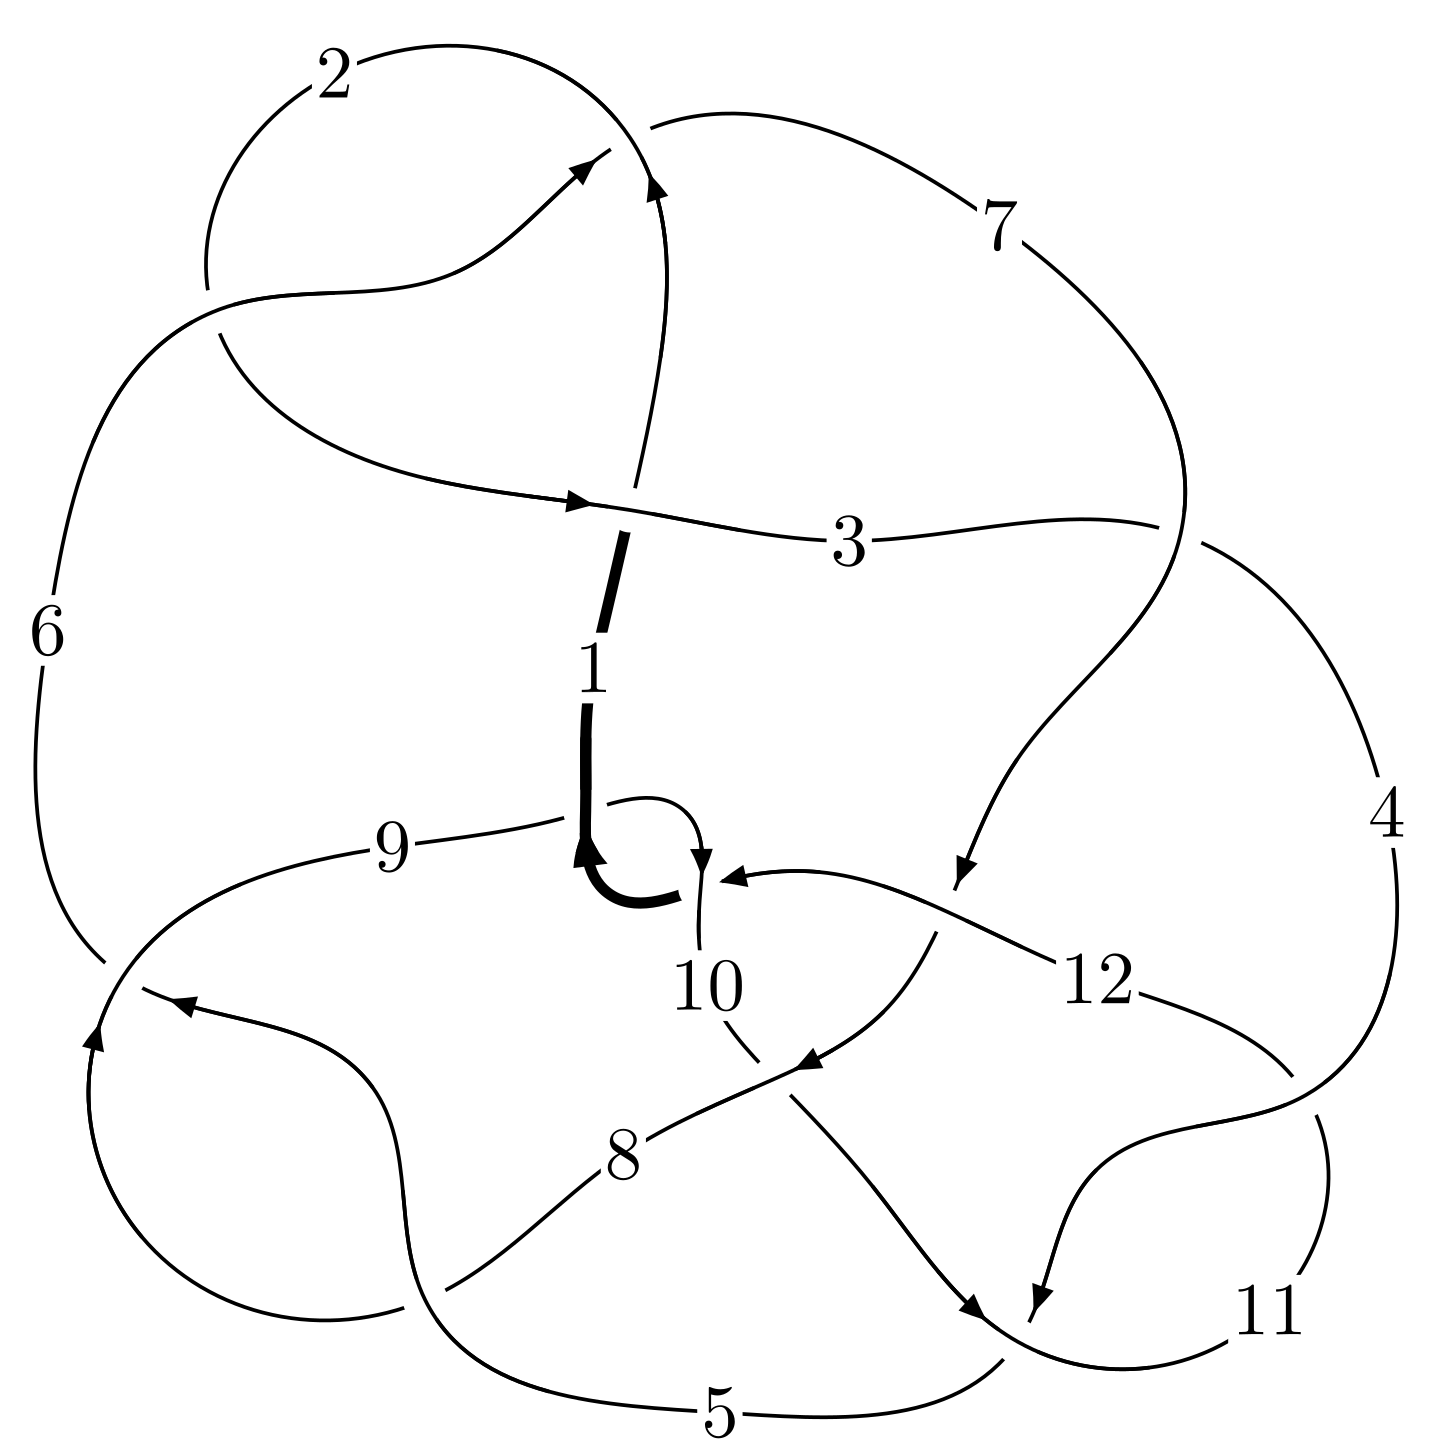
\includegraphics[width=112pt]{../../../GIT/diagram.site/Diagrams/png/1063_12a_0262.png}\\
\ \ \ A knot diagram\footnotemark}&
\allowdisplaybreaks
\textbf{Linearized knot diagam} \\
\cline{2-2}
 &
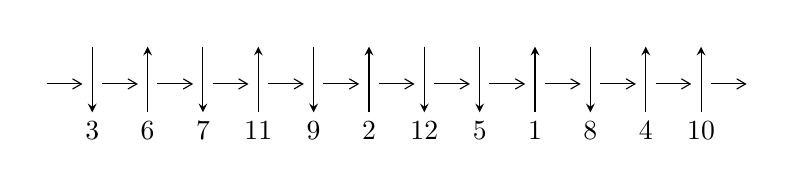
\begin{tikzpicture}[x=20pt, y=17pt]
	% nodes
	\node (C0) at (0, 0) {};
	\node (C1) at (1, 0) {};
	\node (C1U) at (1, +1) {};
	\node (C1D) at (1, -1) {3};

	\node (C2) at (2, 0) {};
	\node (C2U) at (2, +1) {};
	\node (C2D) at (2, -1) {6};

	\node (C3) at (3, 0) {};
	\node (C3U) at (3, +1) {};
	\node (C3D) at (3, -1) {7};

	\node (C4) at (4, 0) {};
	\node (C4U) at (4, +1) {};
	\node (C4D) at (4, -1) {11};

	\node (C5) at (5, 0) {};
	\node (C5U) at (5, +1) {};
	\node (C5D) at (5, -1) {9};

	\node (C6) at (6, 0) {};
	\node (C6U) at (6, +1) {};
	\node (C6D) at (6, -1) {2};

	\node (C7) at (7, 0) {};
	\node (C7U) at (7, +1) {};
	\node (C7D) at (7, -1) {12};

	\node (C8) at (8, 0) {};
	\node (C8U) at (8, +1) {};
	\node (C8D) at (8, -1) {5};

	\node (C9) at (9, 0) {};
	\node (C9U) at (9, +1) {};
	\node (C9D) at (9, -1) {1};

	\node (C10) at (10, 0) {};
	\node (C10U) at (10, +1) {};
	\node (C10D) at (10, -1) {8};

	\node (C11) at (11, 0) {};
	\node (C11U) at (11, +1) {};
	\node (C11D) at (11, -1) {4};

	\node (C12) at (12, 0) {};
	\node (C12U) at (12, +1) {};
	\node (C12D) at (12, -1) {10};
	\node (C13) at (13, 0) {};

	% arrows
	\draw[->,>={angle 60}]
	(C0) edge (C1) (C1) edge (C2) (C2) edge (C3) (C3) edge (C4) (C4) edge (C5) (C5) edge (C6) (C6) edge (C7) (C7) edge (C8) (C8) edge (C9) (C9) edge (C10) (C10) edge (C11) (C11) edge (C12) (C12) edge (C13) ;	\draw[->,>=stealth]
	(C1U) edge (C1D) (C2D) edge (C2U) (C3U) edge (C3D) (C4D) edge (C4U) (C5U) edge (C5D) (C6D) edge (C6U) (C7U) edge (C7D) (C8U) edge (C8D) (C9D) edge (C9U) (C10U) edge (C10D) (C11D) edge (C11U) (C12D) edge (C12U) ;
	\end{tikzpicture} \\
\hhline{~~} \\& 
\textbf{Solving Sequence} \\ \cline{2-2} 
 &
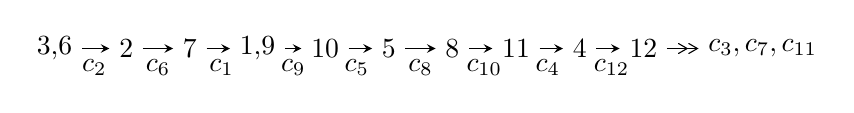
\begin{tikzpicture}[x=23pt, y=7pt]
	% node
	\node (A0) at (-1/8, 0) {3,6};
	\node (A1) at (1, 0) {2};
	\node (A2) at (2, 0) {7};
	\node (A3) at (49/16, 0) {1,9};
	\node (A4) at (33/8, 0) {10};
	\node (A5) at (41/8, 0) {5};
	\node (A6) at (49/8, 0) {8};
	\node (A7) at (57/8, 0) {11};
	\node (A8) at (65/8, 0) {4};
	\node (A9) at (73/8, 0) {12};
	\node (C1) at (1/2, -1) {$c_{2}$};
	\node (C2) at (3/2, -1) {$c_{6}$};
	\node (C3) at (5/2, -1) {$c_{1}$};
	\node (C4) at (29/8, -1) {$c_{9}$};
	\node (C5) at (37/8, -1) {$c_{5}$};
	\node (C6) at (45/8, -1) {$c_{8}$};
	\node (C7) at (53/8, -1) {$c_{10}$};
	\node (C8) at (61/8, -1) {$c_{4}$};
	\node (C9) at (69/8, -1) {$c_{12}$};
	\node (A10) at (11, 0) {$c_{3},c_{7},c_{11}$};

	% edge
	\draw[->,>=stealth]	
	(A0) edge (A1) (A1) edge (A2) (A2) edge (A3) (A3) edge (A4) (A4) edge (A5) (A5) edge (A6) (A6) edge (A7) (A7) edge (A8) (A8) edge (A9) ;
	\draw[->>,>={angle 60}]	
	(A9) edge (A10);
\end{tikzpicture} \\ 

\end{tabular} \\

\footnotetext{
The image of knot diagram is generated by the software ``\textbf{Draw programme}" developed by Andrew Bartholomew(\url{http://www.layer8.co.uk/maths/draw/index.htm\#Running-draw}), where we modified some parts for our purpose(\url{https://github.com/CATsTAILs/LinksPainter}).
}\phantom \\ \newline 
\centering \textbf{Ideals for irreducible components\footnotemark of $X_{\text{par}}$} 
 
\begin{align*}
I^u_{1}&=\langle 
8 u^{32}-16 u^{31}+\cdots+b+9,\;u^{32}-3 u^{31}+\cdots+a+3,\;u^{33}-2 u^{32}+\cdots+2 u-1\rangle \\
\\
\end{align*}
\raggedright * 1 irreducible components of $\dim_{\mathbb{C}}=0$, with total 33 representations.\\
\footnotetext{All coefficients of polynomials are rational numbers. But the coefficients are sometimes approximated in decimal forms when there is not enough margin.}
\newpage
\renewcommand{\arraystretch}{1}
\centering \section*{I. $I^u_{1}= \langle 8 u^{32}-16 u^{31}+\cdots+b+9,\;u^{32}-3 u^{31}+\cdots+a+3,\;u^{33}-2 u^{32}+\cdots+2 u-1 \rangle$}
\flushleft \textbf{(i) Arc colorings}\\
\begin{tabular}{m{7pt} m{180pt} m{7pt} m{180pt} }
\flushright $a_{3}=$&$\begin{pmatrix}1\\0\end{pmatrix}$ \\
\flushright $a_{6}=$&$\begin{pmatrix}0\\u\end{pmatrix}$ \\
\flushright $a_{2}=$&$\begin{pmatrix}1\\u^2\end{pmatrix}$ \\
\flushright $a_{7}=$&$\begin{pmatrix}u\\u^3+u\end{pmatrix}$ \\
\flushright $a_{1}=$&$\begin{pmatrix}u^2+1\\u^2\end{pmatrix}$ \\
\flushright $a_{9}=$&$\begin{pmatrix}- u^{32}+3 u^{31}+\cdots+10 u-3\\-8 u^{32}+16 u^{31}+\cdots+27 u-9\end{pmatrix}$ \\
\flushright $a_{10}=$&$\begin{pmatrix}4 u^{31}-8 u^{30}+\cdots+19 u-8\\-4 u^{32}+6 u^{31}+\cdots+14 u-4\end{pmatrix}$ \\
\flushright $a_{5}=$&$\begin{pmatrix}3 u^{32}-12 u^{31}+\cdots-24 u+9\\2 u^{32}-3 u^{31}+\cdots-15 u+4\end{pmatrix}$ \\
\flushright $a_{8}=$&$\begin{pmatrix}12 u^{32}-35 u^{31}+\cdots-48 u+17\\-6 u^{32}+11 u^{31}+\cdots+10 u-3\end{pmatrix}$ \\
\flushright $a_{11}=$&$\begin{pmatrix}12 u^{32}-15 u^{31}+\cdots+3 u-14\\3 u^{32}-11 u^{31}+\cdots-22 u+12\end{pmatrix}$ \\
\flushright $a_{4}=$&$\begin{pmatrix}u^4+u^2+1\\u^6+2 u^4+u^2\end{pmatrix}$ \\
\flushright $a_{12}=$&$\begin{pmatrix}14 u^{32}-23 u^{31}+\cdots-9 u-8\\2 u^{32}-9 u^{31}+\cdots-20 u+11\end{pmatrix}$\\&\end{tabular}
\flushleft \textbf{(ii) Obstruction class $= 1$}\\~\\
\flushleft \textbf{(iii) Cusp Shapes $= 20 u^{32}-13 u^{31}+159 u^{30}-58 u^{29}+575 u^{28}-25 u^{27}+1135 u^{26}+552 u^{25}+1074 u^{24}+2154 u^{23}-267 u^{22}+4203 u^{21}-1896 u^{20}+4776 u^{19}-1567 u^{18}+2737 u^{17}+1151 u^{16}-350 u^{15}+3593 u^{14}-1677 u^{13}+3251 u^{12}-624 u^{11}+989 u^{10}+1026 u^9-732 u^8+1548 u^7-975 u^6+992 u^5-556 u^4+318 u^3-196 u^2+35 u-42$}\\~\\
\newpage\renewcommand{\arraystretch}{1}
\flushleft \textbf{(iv) u-Polynomials at the component}\newline \\
\begin{tabular}{m{50pt}|m{274pt}}
Crossings & \hspace{64pt}u-Polynomials at each crossing \\
\hline $$\begin{aligned}c_{1}\end{aligned}$$&$\begin{aligned}
&u^{33}-18 u^{32}+\cdots-12 u+1
\end{aligned}$\\
\hline $$\begin{aligned}c_{2}\end{aligned}$$&$\begin{aligned}
&u^{33}-2 u^{32}+\cdots+2 u-1
\end{aligned}$\\
\hline $$\begin{aligned}c_{3}\end{aligned}$$&$\begin{aligned}
&u^{33}+2 u^{32}+\cdots-2 u-1
\end{aligned}$\\
\hline $$\begin{aligned}c_{4}\end{aligned}$$&$\begin{aligned}
&u^{33}+u^{32}+\cdots- u-1
\end{aligned}$\\
\hline $$\begin{aligned}c_{5}\end{aligned}$$&$\begin{aligned}
&u^{33}+3 u^{32}+\cdots+3 u-1
\end{aligned}$\\
\hline $$\begin{aligned}c_{6}\end{aligned}$$&$\begin{aligned}
&u^{33}+2 u^{32}+\cdots+2 u+1
\end{aligned}$\\
\hline $$\begin{aligned}c_{7}\end{aligned}$$&$\begin{aligned}
&u^{33}+2 u^{32}+\cdots+2 u+1
\end{aligned}$\\
\hline $$\begin{aligned}c_{8}\end{aligned}$$&$\begin{aligned}
&u^{33}-3 u^{32}+\cdots+3 u+1
\end{aligned}$\\
\hline $$\begin{aligned}c_{9}\end{aligned}$$&$\begin{aligned}
&u^{33}+5 u^{32}+\cdots+5 u+1
\end{aligned}$\\
\hline $$\begin{aligned}c_{10}\end{aligned}$$&$\begin{aligned}
&u^{33}+6 u^{32}+\cdots+12 u+1
\end{aligned}$\\
\hline $$\begin{aligned}c_{11}\end{aligned}$$&$\begin{aligned}
&u^{33}- u^{32}+\cdots- u+1
\end{aligned}$\\
\hline $$\begin{aligned}c_{12}\end{aligned}$$&$\begin{aligned}
&u^{33}-5 u^{32}+\cdots+5 u-1
\end{aligned}$\\
\hline
\end{tabular}\\~\\
\newpage\renewcommand{\arraystretch}{1}
\flushleft \textbf{(v) Riley Polynomials at the component}\newline \\
\begin{tabular}{m{50pt}|m{274pt}}
Crossings & \hspace{64pt}Riley Polynomials at each crossing \\
\hline $$\begin{aligned}c_{1}\end{aligned}$$&$\begin{aligned}
&y^{33}-2 y^{32}+\cdots+8 y-1
\end{aligned}$\\
\hline $$\begin{aligned}c_{2},c_{6}\end{aligned}$$&$\begin{aligned}
&y^{33}+18 y^{32}+\cdots-12 y-1
\end{aligned}$\\
\hline $$\begin{aligned}c_{3}\end{aligned}$$&$\begin{aligned}
&y^{33}-22 y^{32}+\cdots-26 y-1
\end{aligned}$\\
\hline $$\begin{aligned}c_{4},c_{11}\end{aligned}$$&$\begin{aligned}
&y^{33}+23 y^{32}+\cdots+13 y-1
\end{aligned}$\\
\hline $$\begin{aligned}c_{5},c_{8}\end{aligned}$$&$\begin{aligned}
&y^{33}-37 y^{32}+\cdots+13 y-1
\end{aligned}$\\
\hline $$\begin{aligned}c_{7}\end{aligned}$$&$\begin{aligned}
&y^{33}-10 y^{32}+\cdots+34 y-1
\end{aligned}$\\
\hline $$\begin{aligned}c_{9},c_{12}\end{aligned}$$&$\begin{aligned}
&y^{33}+21 y^{32}+\cdots-13 y-1
\end{aligned}$\\
\hline $$\begin{aligned}c_{10}\end{aligned}$$&$\begin{aligned}
&y^{33}-10 y^{32}+\cdots+30 y-1
\end{aligned}$\\
\hline
\end{tabular}\\~\\
\newpage\flushleft \textbf{(vi) Complex Volumes and Cusp Shapes}
$$\begin{array}{c|c|c}  
\text{Solutions to }I^u_{1}& \I (\text{vol} + \sqrt{-1}CS) & \text{Cusp shape}\\
 \hline 
\begin{aligned}
u &= -0.415757 + 0.879714 I \\
a &= -0.310927 + 0.116953 I \\
b &= \phantom{-}1.245100 + 0.447794 I\end{aligned}
 & -0.28049 - 3.92650 I & -4.28046 + 8.45501 I \\ \hline\begin{aligned}
u &= -0.415757 - 0.879714 I \\
a &= -0.310927 - 0.116953 I \\
b &= \phantom{-}1.245100 - 0.447794 I\end{aligned}
 & -0.28049 + 3.92650 I & -4.28046 - 8.45501 I \\ \hline\begin{aligned}
u &= \phantom{-}0.889089 + 0.341493 I \\
a &= -1.334450 + 0.044982 I \\
b &= -0.835473 - 0.925109 I\end{aligned}
 & -6.37279 - 2.89979 I & -7.35601 + 2.74561 I \\ \hline\begin{aligned}
u &= \phantom{-}0.889089 - 0.341493 I \\
a &= -1.334450 - 0.044982 I \\
b &= -0.835473 + 0.925109 I\end{aligned}
 & -6.37279 + 2.89979 I & -7.35601 - 2.74561 I \\ \hline\begin{aligned}
u &= -0.925009 + 0.139920 I \\
a &= \phantom{-}1.47738 + 0.02503 I \\
b &= \phantom{-}0.640026 - 0.713052 I\end{aligned}
 & -7.59997 + 1.16632 I & -5.62381 + 0.53430 I \\ \hline\begin{aligned}
u &= -0.925009 - 0.139920 I \\
a &= \phantom{-}1.47738 - 0.02503 I \\
b &= \phantom{-}0.640026 + 0.713052 I\end{aligned}
 & -7.59997 - 1.16632 I & -5.62381 - 0.53430 I \\ \hline\begin{aligned}
u &= \phantom{-}0.362523 + 1.024310 I \\
a &= \phantom{-}0.746326 - 0.488114 I \\
b &= \phantom{-}2.02961 + 1.06595 I\end{aligned}
 & -6.88884 - 1.47204 I & -7.24631 - 0.05525 I \\ \hline\begin{aligned}
u &= \phantom{-}0.362523 - 1.024310 I \\
a &= \phantom{-}0.746326 + 0.488114 I \\
b &= \phantom{-}2.02961 - 1.06595 I\end{aligned}
 & -6.88884 + 1.47204 I & -7.24631 + 0.05525 I \\ \hline\begin{aligned}
u &= -0.450656 + 0.786575 I \\
a &= \phantom{-}0.026429 + 0.336633 I \\
b &= -0.047044 + 1.053090 I\end{aligned}
 & \phantom{-}0.012283 + 0.311664 I & \phantom{-}3.64526 - 0.95783 I \\ \hline\begin{aligned}
u &= -0.450656 - 0.786575 I \\
a &= \phantom{-}0.026429 - 0.336633 I \\
b &= -0.047044 - 1.053090 I\end{aligned}
 & \phantom{-}0.012283 - 0.311664 I & \phantom{-}3.64526 + 0.95783 I\\
 \hline 
 \end{array}$$\newpage$$\begin{array}{c|c|c}  
\text{Solutions to }I^u_{1}& \I (\text{vol} + \sqrt{-1}CS) & \text{Cusp shape}\\
 \hline 
\begin{aligned}
u &= \phantom{-}0.699677 + 0.526180 I \\
a &= -0.998558 + 0.221434 I \\
b &= -0.310310 + 0.195387 I\end{aligned}
 & -3.61554 - 3.10551 I & -5.05153 + 3.45408 I \\ \hline\begin{aligned}
u &= \phantom{-}0.699677 - 0.526180 I \\
a &= -0.998558 - 0.221434 I \\
b &= -0.310310 - 0.195387 I\end{aligned}
 & -3.61554 + 3.10551 I & -5.05153 - 3.45408 I \\ \hline\begin{aligned}
u &= -0.461345 + 1.031380 I \\
a &= -0.309219 - 0.530900 I \\
b &= -0.588642 + 0.498459 I\end{aligned}
 & -1.18585 - 3.17980 I & -8.28309 + 4.12212 I \\ \hline\begin{aligned}
u &= -0.461345 - 1.031380 I \\
a &= -0.309219 + 0.530900 I \\
b &= -0.588642 - 0.498459 I\end{aligned}
 & -1.18585 + 3.17980 I & -8.28309 - 4.12212 I \\ \hline\begin{aligned}
u &= \phantom{-}0.319392 + 1.139410 I \\
a &= \phantom{-}0.801591 - 1.128270 I \\
b &= \phantom{-}0.645311 - 0.002396 I\end{aligned}
 & -10.97950 + 0.06682 I & -10.54672 - 0.14143 I \\ \hline\begin{aligned}
u &= \phantom{-}0.319392 - 1.139410 I \\
a &= \phantom{-}0.801591 + 1.128270 I \\
b &= \phantom{-}0.645311 + 0.002396 I\end{aligned}
 & -10.97950 - 0.06682 I & -10.54672 + 0.14143 I \\ \hline\begin{aligned}
u &= \phantom{-}0.567598 + 1.073240 I \\
a &= -0.024768 - 0.681279 I \\
b &= \phantom{-}0.029381 - 0.576170 I\end{aligned}
 & -5.33194 + 8.00776 I & -7.58671 - 6.67740 I \\ \hline\begin{aligned}
u &= \phantom{-}0.567598 - 1.073240 I \\
a &= -0.024768 + 0.681279 I \\
b &= \phantom{-}0.029381 + 0.576170 I\end{aligned}
 & -5.33194 - 8.00776 I & -7.58671 + 6.67740 I \\ \hline\begin{aligned}
u &= \phantom{-}0.213741 + 0.747529 I \\
a &= \phantom{-}0.44378 + 1.36082 I \\
b &= -2.65599 - 0.82648 I\end{aligned}
 & -5.67246 + 4.09164 I & -1.47347 - 8.31889 I \\ \hline\begin{aligned}
u &= \phantom{-}0.213741 - 0.747529 I \\
a &= \phantom{-}0.44378 - 1.36082 I \\
b &= -2.65599 + 0.82648 I\end{aligned}
 & -5.67246 - 4.09164 I & -1.47347 + 8.31889 I\\
 \hline 
 \end{array}$$\newpage$$\begin{array}{c|c|c}  
\text{Solutions to }I^u_{1}& \I (\text{vol} + \sqrt{-1}CS) & \text{Cusp shape}\\
 \hline 
\begin{aligned}
u &= \phantom{-}0.044555 + 0.763029 I \\
a &= \phantom{-}0.26951 + 2.29758 I \\
b &= -1.035990 + 0.506927 I\end{aligned}
 & -8.91211 + 1.56145 I & -7.74657 - 2.97681 I \\ \hline\begin{aligned}
u &= \phantom{-}0.044555 - 0.763029 I \\
a &= \phantom{-}0.26951 - 2.29758 I \\
b &= -1.035990 - 0.506927 I\end{aligned}
 & -8.91211 - 1.56145 I & -7.74657 + 2.97681 I \\ \hline\begin{aligned}
u &= \phantom{-}0.454510 + 1.153340 I \\
a &= \phantom{-}0.284320 - 0.958356 I \\
b &= \phantom{-}0.99905 - 1.93065 I\end{aligned}
 & -3.43511 + 4.06164 I & -1.84707 - 3.29080 I \\ \hline\begin{aligned}
u &= \phantom{-}0.454510 - 1.153340 I \\
a &= \phantom{-}0.284320 + 0.958356 I \\
b &= \phantom{-}0.99905 + 1.93065 I\end{aligned}
 & -3.43511 - 4.06164 I & -1.84707 + 3.29080 I \\ \hline\begin{aligned}
u &= -0.369754 + 1.204530 I \\
a &= -0.469785 - 1.239170 I \\
b &= -0.478866 - 1.069080 I\end{aligned}
 & -11.94570 - 2.89125 I & -9.51390 + 3.40460 I \\ \hline\begin{aligned}
u &= -0.369754 - 1.204530 I \\
a &= -0.469785 + 1.239170 I \\
b &= -0.478866 + 1.069080 I\end{aligned}
 & -11.94570 + 2.89125 I & -9.51390 - 3.40460 I \\ \hline\begin{aligned}
u &= -0.491464 + 1.224780 I \\
a &= -0.115049 - 1.120650 I \\
b &= -1.80600 - 1.71244 I\end{aligned}
 & -11.05150 - 6.20149 I & -8.51895 + 3.78482 I \\ \hline\begin{aligned}
u &= -0.491464 - 1.224780 I \\
a &= -0.115049 + 1.120650 I \\
b &= -1.80600 + 1.71244 I\end{aligned}
 & -11.05150 + 6.20149 I & -8.51895 - 3.78482 I \\ \hline\begin{aligned}
u &= \phantom{-}0.570176 + 1.190950 I \\
a &= -0.053100 - 0.985645 I \\
b &= \phantom{-}1.63829 - 1.28317 I\end{aligned}
 & -9.06173 + 8.29388 I & -8.92407 - 7.11050 I \\ \hline\begin{aligned}
u &= \phantom{-}0.570176 - 1.190950 I \\
a &= -0.053100 + 0.985645 I \\
b &= \phantom{-}1.63829 + 1.28317 I\end{aligned}
 & -9.06173 - 8.29388 I & -8.92407 + 7.11050 I\\
 \hline 
 \end{array}$$\newpage$$\begin{array}{c|c|c}  
\text{Solutions to }I^u_{1}& \I (\text{vol} + \sqrt{-1}CS) & \text{Cusp shape}\\
 \hline 
\begin{aligned}
u &= -0.316420 + 0.565399 I \\
a &= \phantom{-}0.460695 + 1.226470 I \\
b &= \phantom{-}1.380710 + 0.272067 I\end{aligned}
 & \phantom{-}0.381875 - 0.429677 I & -0.97944 - 3.23646 I \\ \hline\begin{aligned}
u &= -0.316420 - 0.565399 I \\
a &= \phantom{-}0.460695 - 1.226470 I \\
b &= \phantom{-}1.380710 - 0.272067 I\end{aligned}
 & \phantom{-}0.381875 + 0.429677 I & -0.97944 + 3.23646 I \\ \hline\begin{aligned}
u &= \phantom{-}0.618289\phantom{ +0.000000I} \\
a &= -1.78836\phantom{ +0.000000I} \\
b &= \phantom{-}0.301684\phantom{ +0.000000I}\end{aligned}
 & -0.353891\phantom{ +0.000000I} & \phantom{-}2.66570\phantom{ +0.000000I}\\
 \hline 
 \end{array}$$\newpage
\newpage\renewcommand{\arraystretch}{1}
\centering \section*{ II. u-Polynomials}
\begin{tabular}{m{50pt}|m{274pt}}
Crossings & \hspace{64pt}u-Polynomials at each crossing \\
\hline $$\begin{aligned}c_{1}\end{aligned}$$&$\begin{aligned}
&u^{33}-18 u^{32}+\cdots-12 u+1
\end{aligned}$\\
\hline $$\begin{aligned}c_{2}\end{aligned}$$&$\begin{aligned}
&u^{33}-2 u^{32}+\cdots+2 u-1
\end{aligned}$\\
\hline $$\begin{aligned}c_{3}\end{aligned}$$&$\begin{aligned}
&u^{33}+2 u^{32}+\cdots-2 u-1
\end{aligned}$\\
\hline $$\begin{aligned}c_{4}\end{aligned}$$&$\begin{aligned}
&u^{33}+u^{32}+\cdots- u-1
\end{aligned}$\\
\hline $$\begin{aligned}c_{5}\end{aligned}$$&$\begin{aligned}
&u^{33}+3 u^{32}+\cdots+3 u-1
\end{aligned}$\\
\hline $$\begin{aligned}c_{6}\end{aligned}$$&$\begin{aligned}
&u^{33}+2 u^{32}+\cdots+2 u+1
\end{aligned}$\\
\hline $$\begin{aligned}c_{7}\end{aligned}$$&$\begin{aligned}
&u^{33}+2 u^{32}+\cdots+2 u+1
\end{aligned}$\\
\hline $$\begin{aligned}c_{8}\end{aligned}$$&$\begin{aligned}
&u^{33}-3 u^{32}+\cdots+3 u+1
\end{aligned}$\\
\hline $$\begin{aligned}c_{9}\end{aligned}$$&$\begin{aligned}
&u^{33}+5 u^{32}+\cdots+5 u+1
\end{aligned}$\\
\hline $$\begin{aligned}c_{10}\end{aligned}$$&$\begin{aligned}
&u^{33}+6 u^{32}+\cdots+12 u+1
\end{aligned}$\\
\hline $$\begin{aligned}c_{11}\end{aligned}$$&$\begin{aligned}
&u^{33}- u^{32}+\cdots- u+1
\end{aligned}$\\
\hline $$\begin{aligned}c_{12}\end{aligned}$$&$\begin{aligned}
&u^{33}-5 u^{32}+\cdots+5 u-1
\end{aligned}$\\
\hline
\end{tabular}\newpage\renewcommand{\arraystretch}{1}
\centering \section*{ III. Riley Polynomials}
\begin{tabular}{m{50pt}|m{274pt}}
Crossings & \hspace{64pt}Riley Polynomials at each crossing \\
\hline $$\begin{aligned}c_{1}\end{aligned}$$&$\begin{aligned}
&y^{33}-2 y^{32}+\cdots+8 y-1
\end{aligned}$\\
\hline $$\begin{aligned}c_{2},c_{6}\end{aligned}$$&$\begin{aligned}
&y^{33}+18 y^{32}+\cdots-12 y-1
\end{aligned}$\\
\hline $$\begin{aligned}c_{3}\end{aligned}$$&$\begin{aligned}
&y^{33}-22 y^{32}+\cdots-26 y-1
\end{aligned}$\\
\hline $$\begin{aligned}c_{4},c_{11}\end{aligned}$$&$\begin{aligned}
&y^{33}+23 y^{32}+\cdots+13 y-1
\end{aligned}$\\
\hline $$\begin{aligned}c_{5},c_{8}\end{aligned}$$&$\begin{aligned}
&y^{33}-37 y^{32}+\cdots+13 y-1
\end{aligned}$\\
\hline $$\begin{aligned}c_{7}\end{aligned}$$&$\begin{aligned}
&y^{33}-10 y^{32}+\cdots+34 y-1
\end{aligned}$\\
\hline $$\begin{aligned}c_{9},c_{12}\end{aligned}$$&$\begin{aligned}
&y^{33}+21 y^{32}+\cdots-13 y-1
\end{aligned}$\\
\hline $$\begin{aligned}c_{10}\end{aligned}$$&$\begin{aligned}
&y^{33}-10 y^{32}+\cdots+30 y-1
\end{aligned}$\\
\hline
\end{tabular}
\vskip 2pc
\end{document}